\chapter{Probas e validación}
\label{chap:validacion}

\lettrine{N}{este} capítulo describirase o proceso de proba e validación do emulador
e os resultados obtidos, tanto contra suites de probas de referencia da comunidade
como con xogos comerciais e en hardware embebido real.

\section{Estratexia de probas}
% tests unitarios dos compoñentes + test roms + validacion manual con xogos
A metodoloxía incremental de desenvolvemento exposta no capítulo~\ref{chap:metodoloxia}
presenta un problema á hora de validar o emulador,
xa que os diversos sistemas do núcleo teñen unha gran dependencia entre si.

Para poder validar o emulador de forma efectiva empregouse unha estratexia de probas en tres niveis:
\begin{itemize}
    \item \textbf{Probas unitarias:} para a validación inicial da \acrshort{cpu}, o compoñente base do emulador e o primeiro en desenvolverse,
    empregáronse probas unitarias sobre as instrucións máis complexas.
    Ao estar cada instrución confinada nun módulo independente e ser cada unha delas sinxela de forma individual,
    esta aproximación resultou efectiva para a detección temperá de erros. No resto de compoñentes este enfoque unitario non é posible,
    xa que son sistemas máis complexos e interdependentes. Ademais, as propias probas poden conter erros, polo que unha mellor aproximación
    é empregar probas amplamente usadas e validadas en hardware real.

    \item \textbf{Validación contra suites de probas de referencia:} unha vez implementados os compoñentes fundamentais para a execución do emulador,
    empregáronse distintos conxuntos de \acrshortpl{rom} deseñados para probar a emulación, amplamente empregados pola comunidade.
    Estes tests teñen unha natureza integral. Aínda que individualmente se centren nun sistema ou compoñente concreto, a súa execución require unha funcionalidade
    mínima en todo o sistema. Os conxuntos empregados expóñense en detalle na sección~\ref{sec:suite_tests}.

    \item \textbf{Validación con xogos comerciais:} despois de conseguir un emulador completo e extensamente validado, a última e máis importante fase de validación consiste
    en executar xogos comerciais reais. Cada un deles pode ter un comportamento diferente e requirir distintas funcionalidades do emulador,
    polo que a súa execución serve como garante definitivo do seu correcto funcionamento. A selección de xogos empregados detállase na sección~\ref{sec:validacion_xogos}.
\end{itemize}


\section{Suite de tests empregadas}
\label{sec:suite_tests}
% empregase cpu blargg, mooneye mbc, dmg-acid2 (manual pero correcto)

Empregáronse tres conxuntos de \acrshortpl{rom} de proba, cada un centrado nunha parte distinta do sistema.
Os tests de Blargg~\cite{blargg} céntranse na \acrshort{cpu} e na \acrshort{apu},
a Mooneye Test Suite~\cite{mooneyetestsuite} nos controladores de bancos de memoria
e dmg-acid2~\cite{dmgacid2} na \acrshort{ppu}.
Os dous primeiros intégranse na batería automática de probas do proxecto,
mentres que o terceiro require comprobación visual e execútase de forma manual.


\subsection{Tests de Blargg}
% blargg serial mostrando o mesmo por pantalla que por serial, tanto diagnostico como resultado final

Os tests de Blargg escriben na pantalla o nome da \acrshort{rom}, os diagnósticos intermedios e o veredicto final,
e envían exactamente esa mesma saída polo porto serie. Buscando a liña \texttt{Passed} no fluxo de bytes recibidos, o test determina se a proba foi superada ou non.

Deste conxunto empréganse tres grupos:
\begin{itemize}
    \item \texttt{cpu\_instrs} valida o comportamento de todo o conxunto de instrucións e das interrupcións, asegurando o correcto funcionamento da \acrshort{cpu}.
    \item \texttt{instr\_timing} comproba a duración en ciclos de cada instrución.
    \item \texttt{dmg\_sound} valida os rexistros e os contadores da \acrshort{apu}.
\end{itemize}

Este último grupo non emprega o porto serie, senón un protocolo baseado na \acrshort{ram} externa do cartucho,
no que a \acrshort{rom} escribe unha sinatura de tres bytes que indica que o resultado xa é válido,
un byte co estado da proba e unha cadea de texto co diagnóstico.
Por iso, a súa execución consulta esas posicións ao final de cada cadro en lugar de agardar por unha transferencia serie.

Estes tests execútanse de forma automática en Github Actions con cada confirmación na rama principal,
de xeito que se garante que o núcleo do emulador non se rompe con cambios posteriores.


\subsection{Mooneye Test Suite}
% mooneye serial enviando a secuencia de fibonacci

A Mooneye Test Suite empregouse para validar os controladores de bancos de memoria.
Para informar do resultado, estas probas empregan un método máis robusto que as de Blargg.
Unha proba superada comunica seis números da secuencia de Fibonacci (3, 5, 8, 13, 21 e 34),
mentres que unha proba fallida comunica o valor \texttt{0x42} repetido seis veces.
Eses valores envíanse polo porto serie e escríbense tamén nos rexistros
\texttt{B}, \texttt{C}, \texttt{D}, \texttt{E}, \texttt{H} e \texttt{L} da \acrshort{cpu}, precedidos e seguidos dunha instrución \texttt{LD B, B}.
Esta instrución non ten ningún efecto en hardware real, pero algúns emuladores empregana como punto de parada para depuración.
Neste traballo descartouse esa vía e a detección faise unicamente polo porto serie,
para manter o núcleo do emulador limpo e fiel ao comportamento da consola.
O listado~\ref{lst:ld-b-b} amosa como o emulador SameBoy~\cite{sameboy} implementa esta instrución.

\begin{lstlisting}[language=C, float=tbp, caption={Uso de \texttt{LD B, B} como punto de parada en SameBoy}, label={lst:ld-b-b}]
// fire the debugger if software breakpoints are enabled
static void ld_b_b(GB_gameboy_t *gb, uint8_t opcode)
{
#ifndef GB_DISABLE_DEBUGGER
    if (gb->has_software_breakpoints) {
        GB_debugger_break(gb);
    }
#endif
}
\end{lstlisting}


\subsection{dmg-acid2}
% dmg-acid2 para a ppu, pero executado de forma manual

A validación da \acrshort{ppu} realízase con dmg-acid2, unha \acrshort{rom} que compón unha imaxe coñecida
exercitando as características do hardware gráfico.
Superando esta proba compróbase o correcto funcionamento do debuxado, aínda que non é exhaustiva
e non garante que todos os xogos funcionen correctamente.
Este é o caso dos que necesitan unha maior precisión, como xa se comentou na sección~\ref{sec:ppu-implementation}.

\begin{figure}[htbp]
  \centering
  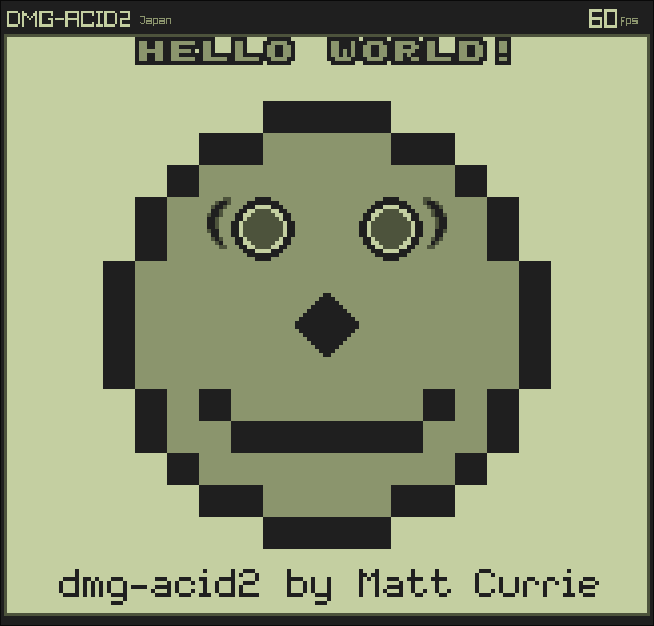
\includegraphics[width=0.4\textwidth]{imaxes/dmg_acid2.png}
  \caption{Resultado correcto da execución de dmg-acid2 no emulador.}
  \label{fig:dmg-acid2}
\end{figure}

A diferenza dos conxuntos anteriores, esta proba non emite o seu veredicto polo porto serie,
polo que require unha revisión manual da imaxe resultante.


\section{Validación con xogos comerciais}
\label{sec:validacion_xogos}
% mostra representativa de cartuchos con diferentes mbcs
% tetris, pokemon, zelda...

Superar as suites de proba non garante que un xogo real funcione, xa que estas comproban comportamentos illados
e non a interacción de todos os compoñentes durante unha partida completa.
Por iso a última fase da validación consistiu en executar xogos comerciais.

A mostra escolleuse entre os xogos máis vendidos do catálogo da \acrshort{dmg},
por seren os máis representativos e tamén os que máis persoas van querer executar no emulador.
Este conxunto é tamén unha mostra representativa do hardware de cartucho emulado,
xa que inclúe exemplos de todos os tipos de cartucho implementados.
A táboa~\ref{tab:xogos-probados} recolle a mostra resultante e o estado de cada xogo.

\begin{table}[htbp]
  \centering
  \resizebox{\textwidth}{!}{%
  \rowcolors{2}{white}{udcgray!25}%
  \begin{tabular}{l|l|c|c|l}
  \rowcolor{udcpink!25}
  \textbf{Xogo} & \textbf{Cartucho} & \textbf{\acrshort{rom}} & \textbf{\acrshort{ram}} & \textbf{Estado} \\\hline
  Pokémon Red        & MBC3 + \acrshort{ram} + batería                  & 1\,MiB   & 32\,KiB & Xogable \\
  Tetris             & Sen controlador                                  & 32\,KiB  & ---     & Xogable \\
  Pokémon Gold       & MBC3 + \acrshort{rtc} + \acrshort{ram} + batería & 2\,MiB   & 32\,KiB & Xogable \\
  Pokémon Crystal    & MBC3 + \acrshort{rtc} + \acrshort{ram} + batería & 2\,MiB   & 32\,KiB & Non compatible \\
  Super Mario Land   & MBC1                                             & 64\,KiB  & ---     & Xogable \\
  Super Mario Land 2 & MBC1 + \acrshort{ram} + batería                  & 512\,KiB & 8\,KiB  & Xogable \\
  Pokémon Pinball    & MBC5 + vibración + \acrshort{ram} + batería      & 1\,MiB   & 8\,KiB  & Xogable \\
  Link's Awakening   & MBC1 + \acrshort{ram} + batería                  & 512\,KiB & 8\,KiB  & Xogable \\
  \end{tabular}}
  \caption{Xogos máis vendidos do catálogo da \acrshort{dmg}, ordenados por vendas, empregados para probar cada controlador.}
  \label{tab:xogos-probados}
\end{table}

A proba de cada xogo consistiu en xogar as súas zonas iniciais comprobando que o debuxado, a entrada e o audio funcionan correctamente,
e, nos cartuchos con batería, en gardar a partida, pechar o emulador e recuperala nunha execución posterior.
Todos os xogos da mostra son xogables sen problemas relevantes, agás algún fallo gráfico menor puntual.

A única excepción é Pokémon Crystal, que non é compatible por deseño,
xa que se trata dun cartucho exclusivo de Game Boy Color, que tampouco se executa nunha \acrshort{dmg} real,
polo que queda fóra do alcance deste traballo.
Si funcionan, en cambio, os xogos retrocompatibles como Pokémon Gold,
que detectan que se están a executar nunha consola monocroma e se adaptan a ela.
Estes xogos escriben igualmente nos rexistros propios de Game Boy Color,
que na \acrshort{dmg} simplemente non teñen efecto, tal e como se describiu no capítulo~\ref{chap:implementacion}.

Ademais desta mostra, ao longo do desenvolvemento probáronse outros xogos de forma máis puntual.
Esta fase é a que permite detectar erros nas partes que as suites de proba non cobren,
como a composición de cadros con moitos obxectos ou o encaixe entre a execución da \acrshort{cpu} e o avance do resto de compoñentes.

